\chapter{Navigation}\label{cha:navigation}
Ce chapitre décrit le fonctionnement de la carte mobile en tant qu'aide à la navigation.
Il décrit  les interactions possibles avec la carte et les informations de navigations qui peuvent être superposées.

\section{Éléments de la carte mobile}

\begin{maxipage}
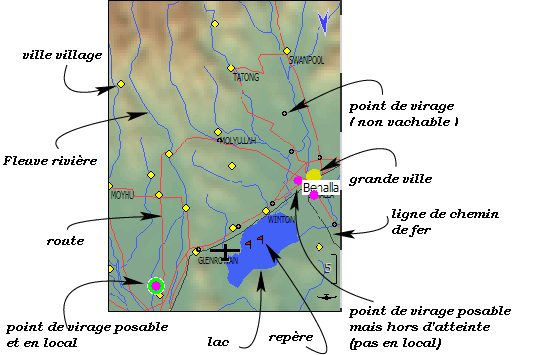
\includegraphics[angle=0,width=0.9\linewidth,keepaspectratio='true']{figures/fig-map.png}
\end{maxipage}

Sont représentés sur la carte:
\begin{enumerate} 
\item planeur, vent, profil du thermique, indicateur d'arrivée
\item Terrain, relief et altitude du terrain
\item Topographie, rivières, routes, agglomérations
\item Waypoints, aérodromes, terrains vachables 
\item Le circuit en cours,zones d'observation , points de virage
\item Le cap à suivre (ou route à suivre\footnote{Direction menant au prochain point de virage: la  {\em trajectoire}, voir Section~\ref{sec:route}.}) 
\item Espace aérien
\item Repères, historique des thermiques, trace au sol
\item Zone atteignable en plané\footnote{La zone atteignable en plané est aussi nommée {\em local}, comme décrit dans la  section~\ref{sec:reach}.}
\end{enumerate}
La carte est représentée dans un système de coordonnées projetées, l'échelle est modifiable (zoom, dézoom) et la carte peut être déplacée dans toutes les directions. Toutes les fonctionnalités de navigation prennent en compte la courbure de la terre.

\section{Symbole du planeur, orientation de la carte}
Le symbole du planeur montre sa position sur la carte. L'orientation du planeur indique le cap estimé du planeur.
La carte est positionnée de 3 façons possibles: 
\begin{enumerate}
\item [-] Nord en haut
\item [-] Trajectoire vers le haut
\item [-] Destination vers le haut
\end{enumerate}
Le paramétrage  \config{orientation} permet de définir un autre mode d'orientation durant les spirales. Ceci est très utile pour ne pas être désorienté en regardant la carte en spirale. Le mode "destination vers le haut" en spirale facilite le choix de la direction à prendre lors de la sortie du thermique.

Quand les modes trajectoire ou destination vers le haut sont utilisés en spirale, le symbole du planeur est au milieu de l'écran même si la position du symbole planeur a été configurée autrement.  En transition, les modes trajectoire et destination vers le haut permettent de positionner le symbole du planeur au bas de l'écran (à environ 20\% de la hauteur de l'écran), permettant une bonne visualisation de la carte devant le planeur. Cette position par apport au bord bas de l'écran est paramétrable dans le menu Config./Options Système/Afficher la carte/Orientation.Voir \config{gliderposition}.

\section{Zoom et mise à l'échelle}\label{sec:zooming}
Le changement d'échelle de la carte sur PC, PNA et Pocket PC:
\begin{enumerate}
\item Appui/clic sur une partie blanche de la carte pour la sélectionner si elle ne l'est pas déjà.
Puis utiliser la roulette de la souris ou les flêche haut/bas du Pocket PC pour zoomer/dézoomer.
\item Un PNA muni d'un bouton roulette permet aussi de zoomer/dézoomer.
\item Les terminaux Android sont munis d'un bouton bascule permettant de changer d'échelle.(il permet normalement de régler le volume).Situé sur le côté du terminal, il n'est guère accessible en vol lorsque l'appareil est dans un support générique.
\item Vous pouvez changer d'échelle par simple geste. Le geste  \gesture{Haut/Bas}
``Appui + Haut'' zoom, ``Appui + Bas'' dézoom.
\item Ou sélectionner la fonction à l'aide des menus.:
\begin{quote}
\bmenu{Affich.}\blink\bmenu{Zoom} et \bmenu{Affich}\blink\bmenu{Dézoom}
\end{quote}
\end{enumerate}
Sur un Altair, le bouton de rotation peut être utilisé pour la mise à l'échelle.
L'échelle est visible dans l'angle inférieur gauche de la carte mobile.
La distance indiquée est la distance sur la carte comprise entre les deux bords de l'écran.
\marginpar{\includegraphics[angle=0,width=0.4\linewidth,keepaspectratio='true']{figures/zoom.png}}

Utilisateurs de Compaq Aero: si vous activez les touches de jeux Compaq Aero (avec le Q-menu) les deux boutons centraux deviennent alors les touches Haut/Bas.
 
Deux paramétrages du zoom sont possibles: l'un pour le vol en spirale et l'autre pour les transitions ou les arrivées. C'est "Zoom en spirale" du menu Config./Options Système/Afficher la carte/Orientation  \config{circlingzoom}. Par défaut le  "Zoom en spirale" est défini entre 2,5km et 5km en fonction de la taille de l'écran. Quand l'utilisateur zoom/dézoom, ceci affecte uniquement le mode de zoom courant. Ceci fait qu'en sortant de spirale, l'utilisateur retrouve l'échelle qu'il avait avant, en transition. Si  "Zoom en spirale" est sur "off"  il n'y a alors qu'un seul niveau de zoom pour les différentes phases de vol.

Zoom Auto. permet de zoomer automatiquement à l'approche d'un point de virage, afin de garder celui-ci à l'écran.  Quand Zoom Auto est actif, 'AUTO 'apparait au dessus de l'échelle actuelle dans l'angle inférieur gauche de l'écran. L'utilisateur peut toujours zoomer/dézoomer s'il le souhaite. Le contrôle du zoom passe alors automatiquement en mode Zoom Manuel.
\marginpar{\includegraphics[angle=0,width=0.4\linewidth,keepaspectratio='true']{figures/zoomauto.png}}
Pour passer d'un mode de zoom à l'autre, utilisez le menu:
\begin{quote}
\bmenu{Affich.}\blink\bmenu{Zoom Auto} 
\end{quote}
Quand un point de virage change (automatiquement, à l'aide du gestionnaire de circuit, ou par changement manuel du prochain point de virage), Zoom Auto règle l'affichage afin de faire apparaitre à l'écran le prochain point de virage.
En spirale si une ascendance est détectée, alors le thermique est centré sur la carte tout en faisant en sorte que le planeur soit toujours visible.

\section{Déplacement de la carte}\label{sec:panning}
Le mode déplacement panoramique de la carte permet de se déplacer sur toute la carte tout en gardant la même échelle. Ceci est très utile lors de la préparation des circuits.
\begin{enumerate}
\item Activation du mode déplacement par pression (ou par geste)  \gesture{Haut - Droite - Bas - Gauche}
\begin{quote}
\bmenu{Affich.}\blink\bmenu{Panor. ON}
\end{quote}

\item Le déplacement de la carte se fait en tirant dans n'importe quelle direction à l'aide du doigt, de la souris ou des touches permettant de déplacer le curseur. Pour Altair ceci s'effectue à l'aide des  touches intérieur/extérieur du bouton de rotation.
\item Le mode panoramique se désactive en utilisant;
\begin{quote}
\bmenu{Panor. OFF}
\end{quote}
\end{enumerate} 

\sketch{figures/pan.png}
Quand le mode panoramique est activé, 'PAN' s'affiche au dessus de l'échelle. Les coordonnées GPS affichées en haut et à droite sont celles de la petite croix du centre. Si la carte topographique est chargée, l'altitude du point est affichée.
Un menu spécifique apparait en mode panoramique facilitant l'exploration de la carte et la préparation des circuits.

\section{Points de virage} \label{sec:waypoint-schemes}
Les points de virage sont représentés différemment suivant leur type: la principale caractéristique étant "vachable" ou "non vachable".
Les points de virage sont représentés ci-dessous. Il existe 3 ensembles de symboles pour les points de virages vachables.\config{waypointicons}

\begin{tabular}{c|c|cc|cc|}
Symboles &\begin{sideways}WP simple\end{sideways}
&\begin{sideways}WP vachable\end{sideways}
&\begin{sideways}WP en local\end{sideways}
&\begin{sideways}aérodrome\end{sideways}
&\begin{sideways}WP en local\end{sideways}\\
\hline
Violets &
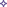
\includegraphics[width=0.5cm]{icons/map_turnpoint.pdf} &

\includegraphics[width=0.8cm]{icons/winpilot_landable.pdf} &

\includegraphics[width=0.8cm]{icons/winpilot_reachable.pdf} &
\colorbox{white}{
\includegraphics[width=0.8cm]{icons/winpilot_landable.pdf}}
& 
\includegraphics[width=0.8cm]{icons/winpilot_reachable.pdf} \\
\hline
N/B & 
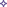
\includegraphics[width=0.5cm]{icons/map_turnpoint.pdf} &

\includegraphics[width=0.9cm]{icons/alt_landable_field.pdf} &
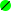
\includegraphics[width=0.9cm]{icons/alt_reachable_field.pdf} &
\colorbox[rgb]{0.94,0.94,0.94}{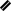
\includegraphics[width=0.9cm]{icons/alt_landable_airport.pdf}}
& 
\includegraphics[width=0.9cm]{icons/alt_reachable_airport.pdf} \\
\hline
Oranges & 
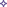
\includegraphics[width=0.5cm]{icons/map_turnpoint.pdf} &

\includegraphics[width=0.9cm]{icons/alt2_landable_field.pdf} &
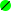
\includegraphics[width=0.9cm]{icons/alt_reachable_field.pdf} &
\colorbox{white}{
\includegraphics[width=0.9cm]{icons/alt2_landable_airport.pdf}}
& 
\includegraphics[width=0.9cm]{icons/alt_reachable_airport.pdf} \\
\hline
\end{tabular}
\\

Les poins de virages peuvent être nommés suivant différentes règles \config{labels}  et suivant leur accessibilité. 
XCSoar calcule en permanence  les points de virage qui sont en local en prenant en considération le vent estimé. L'altitude estimée d'arrivée {\em au dessus de l'altitude de sécurité d'arrivée} des points de virages atteignables (en local) est affichée à côté du point de virage. L'altitude estimée d'arrivée est calculée à partir de la finesse réalisée et de la valeur du calage MacCready du circuit actif\config{reachpolar}, ou la valeur MacCready de sécurité.

\section{Circuit en cours(actif)}
Le circuit en cours est représenté sur la carte par une ligne vert sombre pointillée.
Les lignes de départ/arrivée et les points de virage définis pour le circuit en cours sont représentés en jaune.
Un cercle est toujours représenté autour des point de départ et d'arrivée. Une ligne (avec secteur) est affichée si ces points sont de type ligne. 

Une ligne noire est affichée en permanence du planeur vers le prochain point de virage du circuit en cours. Cette ligne peut pointer directement vers le point de virage, ou bien donner le chemin  de contournement {\em trajectoire} d'un terrain ou d'un espace aérien: décrit en détail dans la Section~\ref{sec:route}.

\begin{center}
\begin{tabular}{c c c}
{\it Départ/arrivée} & {\it Secteur} & {\it Cylindre} \\
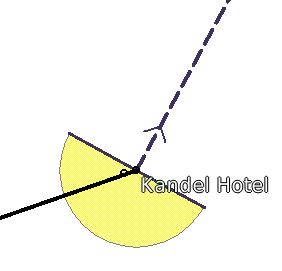
\includegraphics[angle=0,width=0.3\linewidth,keepaspectratio='true']{figures/cut-startfinish.png} &
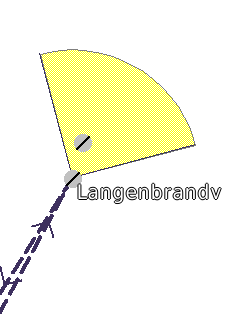
\includegraphics[angle=0,width=0.3\linewidth,keepaspectratio='true']{figures/cut-sector.png} &
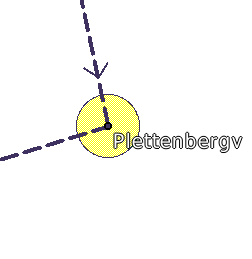
\includegraphics[angle=0,width=0.3\linewidth,keepaspectratio='true']{figures/cut-barrel.png} \\
\end{tabular}
\end{center}

\section{Relief et topographie}\label{sec:terrain_topo}

Les éléments topographiques affichés sur la carte sont:
\begin{itemize}
\item Routes principales, en rouge.
\item Fleuves et rivières, en bleu.
\item Grandes étendues d'eau (lacs), zones bleues
\item Grandes villes, zones jaunes
\item Villages et petites villes, petits diamants jaunes ou nom seul.
\end{itemize}
Les villes et villages sont écrits en italique.

Le relief est coloré en fonction de l'altitude et optionnellement ombré suivant la direction du soleil ou par les pentes porteuses. Les reliefs non valides ou sous le niveau de la mer sont représentés en bleu.

Le relief est ombré pour améliorer sa lisibilité. Par défaut l'éclairage virtuel utilisé est celui du cap du vent estimé. Les faces les plus claires sont les faces portantes, les faces sombres sont sous le vent. L'ombrage et la clarté globales sont paramétrables. Le développement d'un éphéméride du soleil est en cours. Pour configurer l'ombrage et la clarté du relief voir \config{shading}.

L'affichage du relief et de la topographie peuvent être activés/désactivés par les menus:
\begin{quote}
\bmenu{Affich. 2}\blink\bmenu{Relief On} \\
\bmenu{Affich. 2}\blink\bmenu{Topo. On}
\end{quote}

\begin{center}
\begin{tabular}{c c}
Topographie & Relief \\
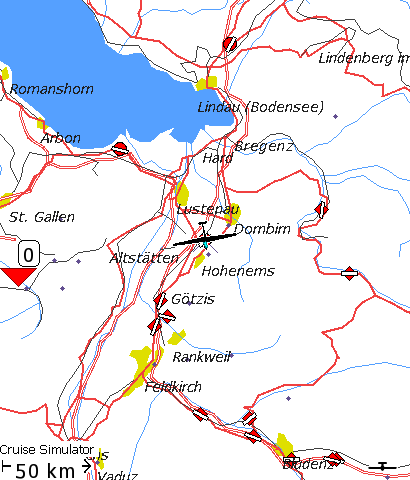
\includegraphics[angle=0,width=0.4\linewidth,keepaspectratio='true']{figures/cut-topo.png} &
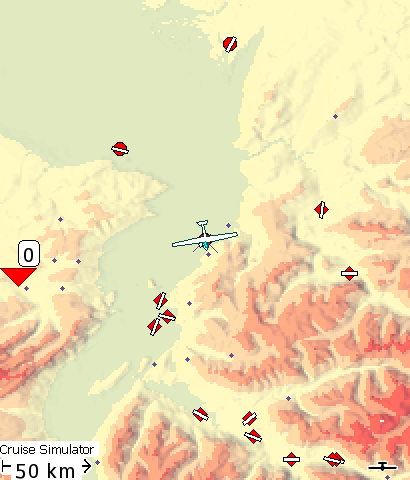
\includegraphics[angle=0,width=0.4\linewidth,keepaspectratio='true']{figures/cut-terrain.png} \\
\end{tabular}
\end{center}

Si la carte de relief n'est pas chargée(ou si son affichage est sur Off), le fond de la carte est blanc. Tout relief sous le niveau de la mer est représenté en bleu. Si vous volez en dehors de la carte "relief"  le fond de carte est aussi blanc.

\subsection*{Étiquettes sur la carte}\label{sec:maplabels}

L'écran peut contenir trop d'information et être peu lisible. Il est possible de ne plus montrer les textes  topographiques et toutes les infos ne concernant pas le circuit en utilisant:
\begin{quote}
\bmenu{Affich. 2}\blink\bmenu{Etiquettes Circuit}
\end{quote}

D'autres options sont disponibles:

\jindent{\bmenut{Etiquettes}{Circuit \& Terrains posables}}{ Montre les noms des points de virage du circuit en cours et de tout les terrains posables (basé sur les attributs des points de virages du fichier de points de virage). Les autres points de virage sont représentés mais sans étiquette. }
\jindent{\bmenut{Etiquettes}{Circuit}}{ Montre uniquement les noms des points de virage du circuit en cours}
\jindent{\bmenut{Etiquettes}{Tous}}{ Montre les noms de tous les points de virage. }
\jindent{\bmenut{Etiquettes}{Aucun}}{ Aucun nom de points de virage. }

Le format des étiquettes est touours paramétrable dans le menu\config{labels} de configuration Config./Options Système/Afficher la carte/Waypoints. 

\section{Trace sol}\label{sec:trail}

Une 'trace sol' optionnelle est dessinée sur la carte et montre le trajet passé du planeur. La couleur et l'épaisseur de la trace est configurable en fonction de la hauteur ou de la valeur du variomètre. \config{snailtype} 

\begin{center}
\includegraphics[angle=0,width=0.8\linewidth,keepaspectratio='true']{figures/snail.pdf}
\end{center}

Si un Vega ou un vario "intelligent" est connecté avec un sotie "Netto", la valeur Netto est utilisée. Alors la couleur et l'épaisseur de la trace sol représente la vitesse verticale de la masse d'air à la place de celle du planeur.

La longueur de la trace sol peut être désactivée, courte (environ 10 minutes) ou bien longue (environ 1 heure) ou encore infinie (vol complet). Ce réglage peut être permanent en utilisant le menu de configuration \config{snailtrail} ou temporaire à l'aide du menu:
\begin{quote}
\bmenu{Affich. 2}\blink\bmenu{Trace On} \\
\bmenu{Affich. 2}\blink\bmenu{Trace Court} \\
\bmenu{Affich. 2}\blink\bmenu{Trace Long} \\
\bmenu{Affich. 2}\blink\bmenu{Trace Complet} \\
\bmenu{Affich. 2}\blink\bmenu{Trace Off}
\end{quote}

Pour tout les modes de trace, en spirale la trace est courte afin de laisser la carte lisible.

Dans le but d'aider au centrage des ascendances quand il y a du vent, la trace sol en spirale peut être déviée artificiellement en fonction du vent (dérive compensée en spirale). De cette façon la trace sol fait référence au vent et non plus au sol. Comme le thermique se déplace aussi avec le vent, la trace sol donne une meilleure indication de la position du thermique par rapport au planeur.

La figure suivante en montre l'exemple. Quand la dérive compensée en spirale est activée (figure de droite) le planeur semble tourner dans une colonne verticale plutôt que dans une colonne oblique (figure de gauche).

\begin{center}
\includegraphics[angle=0,width=0.8\linewidth,keepaspectratio='true']{figures/traildrift.png}
\end{center}

L'activation de la "dérive compensée en spirale" se fait dans le menu de configuration du vent  \config{traildrift}.  La compensation n'a lieu qu'en spirale. La trace sol en transition n'en tiens pas compte.
Le paramétrage peut se faire aussi avec le menu Options Vent:
\begin{quote}
\bmenu{Config.}\blink\bmenu{Options Vent}
\end{quote}

L'affichage de la dérive est aussi utile afin de montrer plus clairement l'effet du du cisaillement du vent sur les thermiques.

La épaisseur de la trace sol peut être agrandie en fonction de la valeur du vario\config{trailscaled}.

\section{Marques}\label{sec:markers}

Les marques sont représentées par de petits drapeaux (a). Les marques peuvent être placée à la main en appuyant sur un bouton ou automatiquement. Un exemple d'utilisation en mode automatique est de placer une marque à chaque entrée en mode spirale, une façon simple de repérer tout les thermiques du vol.

Les marques ne sont pas conservées sur la carte quand on éteint XCSoar. Les marques sont ajoutées au fichier de marques  \verb|xcsoar-marks.txt|.

Pour poser une marque utiliser le menu: 
\begin{quote}
\bmenu{Nav. 2}\blink\bmenu{Marquer}
\end{quote}

\section{Marques de thermiques}

En montée dans les thermiques, des marques sont crées automatiquement et stockées \sketch{figures/thermalhistory.png} jusqu'à la fin du vol. En sélectionnant la marque sur la carte vous obtenez le panel suivant:
\begin{center}
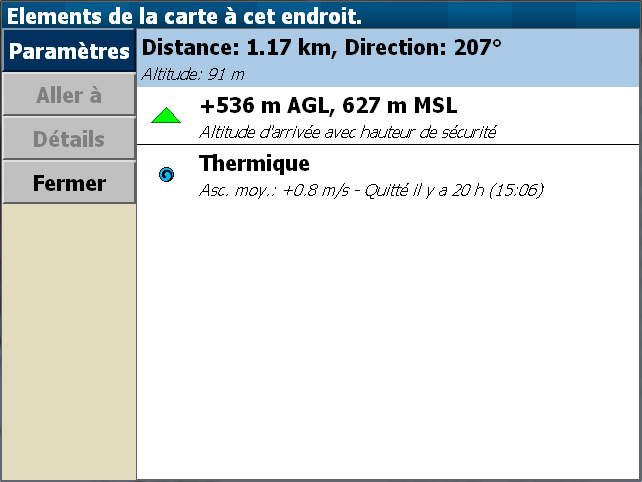
\includegraphics[angle=0,width=0.8\linewidth,keepaspectratio='true']{figures/marque_panel.png}
\end{center}

\section{Zone atteignable en plané }\label{sec:reach}

La limite de la zone atteignable en plané est représentée par une ligne pointillée noire.
Elle indique le contour de la zone que peut atteindre le planeur en tenant compte de la topographie et du relief.
 
Les calculs peuvent être configurés  \config{turningreach} avec 2 niveaux de détail:
\begin{description}
\item[En ligne droite] Calcul la limite de Zone atteignable en finale dans toutes les directions, en ligne droite. La limite est alors une courbe fermée autour du planeur.
\begin{center}
\includegraphics[angle=0,width=1.0\linewidth,keepaspectratio='true']{figures/reach1.png}
\end{center}

\item[Contourne] Si le mode contournement est choisi alors le relief et les espaces aériens sont pris en compte. Le contournement des obstacles est calculé.\footnote{le maximum de virages est de 3, et aucun virage supérieur à 90 degrés}  La Zone atteignable est alors une courbe fermée autour du planeur mais elle peut comporter des "trous" indiquant des zones hors de portée (sommets montagneux) sans reprendre de l'altitude.
\begin{center}
\includegraphics[angle=0,width=1.0\linewidth,keepaspectratio='true']{figures/reach2.png}
\end{center}

\end{description}

L'affichage peut être configuré afin de rendre floue la zone non atteignable. \config{gliderange} 

Le calcul de la trajectoire de zone atteignable en plané prend en compte les paramètres de sécurité configurés.  Voir Section~\ref{sec:safety-heights}.

Si il y a un obstacle, une croix rouge apparait sur la carte à l'endroit de la collision/violation. Si une destination est sélectionnée le calcul est effectué le long du trajet menant à cette destination.

Si "zone atteignable en plané" est activée, alors le mode "Abandon de circuit" prend en compte les points encore "en local". Ceux-ci font partie de la liste des "Dégagements" et sont affichés sur la carte comme atteignables.

Il faut noter que les calculs du circuit en cours ne sont pas impactés par les calculs de zone atteignable en plané. Par exemple la flèche d'altitude nécessaire pour terminer le parcours ou les données du circuits affichées dans les boîtes d'information ne sont pas affectés par les calculs "zone atteignable en plané".

Les calculs de "zone atteignable en plané" sont utilisés pour: la trace au sol de la zone de local, la hauteur d'arrivée sur des points posables, par le mode "Abandon de circuit " et par les ordres de dégagement. Les performances du planeur et le calage du MacCready utilisés pour ces calculs sont paramétrables \config{reachpolar}:
\begin{description}
\item[Circuit] La valeur de calage du MC pour le circuit.
\item[MC de sécurité] Une valeur faible de calage du MC doit être entrée par le pilote afin de refléter des performances légèrement dégradées par rapport aux performances maximales du planeur. 

\end{description}


\section{États}\label{sec:flight-status}

Le panel des États comporte plusieurs onglets regroupant l'accès à des informations du vol, du circuit, des règles, des temps et durées ainsi qu'à des informations système. Ce sont des informations et ne sont donc pas modifiables par l'utilisateur.
On y accède en faisant un "S à angles droits" sur l'écran ou par les boutons menus sous:\gesture{Gauche - Bas - Droite - Bas - Gauche}
\begin{quote}
\bmenu{Info. 2}\blink\bmenu{Etats}
\end{quote}
On sélectionne ensuite l'un des onglets.

\subsection*{Localisation}
% \sketch{figures/status-flight.png}
Le panel Etats 'Flight' donne la position GPS, l'altitude, le gain d'altitude maximal réalisé, le point de virage le plus proche, son cap et sa distance. Cette fonctionnalité est intéressante pour communiquer votre position à d'autres!! (vos dépanneurs?)
\begin{center}
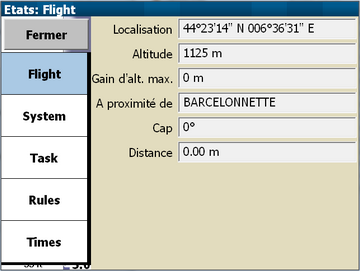
\includegraphics[angle=0,width=0.7\linewidth,keepaspectratio='true']{figures/status-flight.png}
\end{center}

\subsection*{Times}
Ce panel donne l'heure locale, la date et l'heure UTC, la durée du vol, l'heure de décollage et d'atterrissage, et le coucher du soleil.
\begin{center}
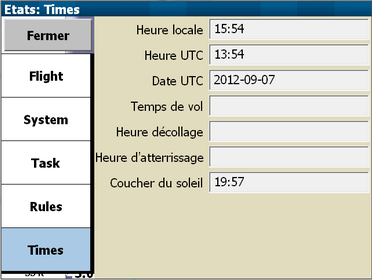
\includegraphics[angle=0,width=0.7\linewidth,keepaspectratio='true']{figures/status-times.png}
\end{center}
REMARQUE: les valeurs affichées dans les panels 'États' sont statiques! Les valeurs affichées sont celles valables à l'ouverture de l'onglet sélectionné. Pour avoir la valeur à jour, il faut ouvrir un autre onglet et réouvrir l'onglet désiré. 

\section{Trajectoire}\label{sec:route}
Entre l'aéronef et la destination en cours, XCSoar peut calculer la trajectoire, en 3 dimensions,  en considérant le relief et les espaces aériens. L'altitude de la destination est calculée comme les points d'arrivée. Elle peut-être supérieure pour les points intermédiaires du au fait de la prise en compte des reliefs ou des espaces aériens.
Le calcul de la trajectoire fonctionne en mode circuit normal, en mode 'Abandon' et en mode 'Aller à'.
%XCSoar can plan paths around terrain and airspace obstacles in three
%dimensions from the aircraft to the destination.  Such a path is known
%as a route.  The height of the destination is the arrival height for
%final waypoints, or may be higher for intermediate waypoints, as
%dictated by the task system as required to complete the task.  Route
%planning functions in normal ordered task mode, abort mode and goto
%mode.

\begin{center}
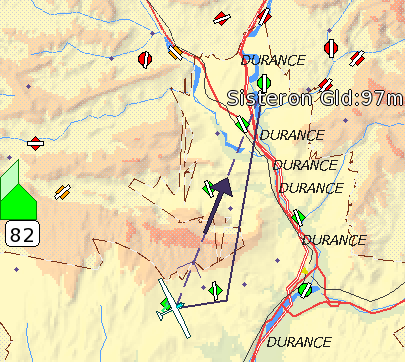
\includegraphics[angle=0,width=1.0\linewidth,keepaspectratio='true']{figures/route3.png}
\end{center}

Le calcul  d'optimisation des trajectoires est basé sur les performances (la polaire) du planeur. Elles sont optimisées par rapport au temps de vol. Le calcul d'optimisation des trajectoires est inactif par défaut. Pour le paramétrer quatre valeurs sont disponibles\config{routemode}. :
\begin{description}
\item[Aucun] Calcul d'optimisation des trajectoires inactif.
\item[Relief] La trajectoire évitera le relief.
\item[Espace Aérien]  La trajectoire évitera les espaces aériens.
\item[Les 2] La trajectoire évitera les espaces aériens et le relief.
\end{description}

Pour les calculs, la hauteur minimum par rapport au relief (la garde au sol, un peu comme le pied pilote chez les marins) est paramétrable\config{safetyterrain}.  Il n'y a pas de distance minimum latérale prise en compte.
Une trajectoire optimisée peut indiquer une altitude d'arrivée supérieure à l'altitude minimum d'arrivée non optimisée: par exemple si la destination se trouve derrière une montagne.

Les espaces aériens sont évités horizontalement par un "matelas" (buffer) d'environ 250 mètres. Il n'y a pas de "matelas" vertical imposé. Des trajectoires valides peuvent passer au-dessus et au-dessous d'espaces aériens.

Pour les trajectoires optimisées, si le calage MacCready est positif, le calcul de la trajectoire peut autoriser ou non les montées entre la position du planeur et la destination.\config{routeceiling}.

Le calcul de trajectoire peut aussi permettre de limiter le plafond de celle-ci. Il peut être limité au plafond le plus élevé entre 500 mètres au dessus de l'altitude courante et le plafond des thermiques\config{routeceiling}. Si ce mode de calcul n'est pas activé, le plafond de la trajectoire n'est pas limité.

%Pour les trajectoires calculées, si le MacCready est positif, les prises d'ascendances sont autorisées en option \config{routeceiling}. Le sommet de l'ascendance peut être alors limité à 500 m au dessus du plus haut des plafonds de départ et d'arrivée, ou bien accru de la valeur du plafond défini dans les paramètres\config{routeceiling}. La montée au-dessus 
%If MacCready is positive, then climbs are optionally allowed
%\config{routeceiling} in the computed routes.  The top of the climb
%may be limited to 500 m above the heigher of the start and destination
%ceiling, or increased to the ceiling defined by the thermal ceiling
%\config{routeceiling}.  Climbs above the higher of the start and
%destination altitude are penalised by a slower climb rate than the
%actual MacCready value.

Les approximations et limitations du calcul de trajectoire sont les suivantes:
\begin{itemize}
\item Quand les montées sont nécessaires (et autorisées) pour atteindre le prochain point de virage, les montées sont considérées comme ayant lieu en début de trajectoire.
\item Les transitions en montées sont considérées comme étant à altitude constante, et équivalent à une série de petites montées réparties le long de la trajectoire.
\item Le long de la trajectoire, les virages de plus de 90 ° ne sont pas autorisés.
\item Si l'algorithme de calcul de trajectoire ne réussi pas, le calcul repasse en mode ??? qui se base sur la position actuelle du planeur et du point de destination.
\end{itemize}

